% This is text associated with the open textbook "Open Electromagnetics"
% See immediately below for author, date
% This work is licensed under the Creative Commons Attribution-ShareAlike 4.0 International License. (CC BY-SA 4.0) 
% To view a copy of the license, visit http://creativecommons.org/licenses/by-sa/4.0/

%ORB TITLE Transmission Lines as Two-Port Devices
%ORB AUTHOR 0        # S.W. Ellingson, Virginia Tech (ellingson@vt.edu)
%ORB DATE 20180802   # yyyymmdd
%ORB ABSTRACT Transmission Lines as Two-Ports

\label{m0077_Transmission_Lines_as_Two-Ports} % <-- Must match name of this file and module directory name.  Don't mess with this!
\index{transmission line!two-port representation|(}

Figure~\ref{m0077_fTransmission_line_symbols} shows common ways to represent transmission lines in circuit diagrams.
In each case, the source is represented using a Th\'{e}venin equivalent circuit 
\index{Th\'{e}venin equivalent circuit}
consisting of a voltage source $V_S$ in series with an impedance $Z_S$.\footnote{For a refresher on this concept, see ``Additional Reading'' at the end of this section.}  In transmission line analysis, the source may also be referred to as the \emph{generator}.
\index{generator}
The termination on the receiving end of the transmission line is represented, without loss of generality, as an impedance $Z_L$. 
This termination is often referred to as the \emph{load}, although in practice it can be any circuit that exhibits an input impedance of $Z_L$.
%
\begin{figure}[b!]
\begin{center}
\pdftooltip{{  % note double braces
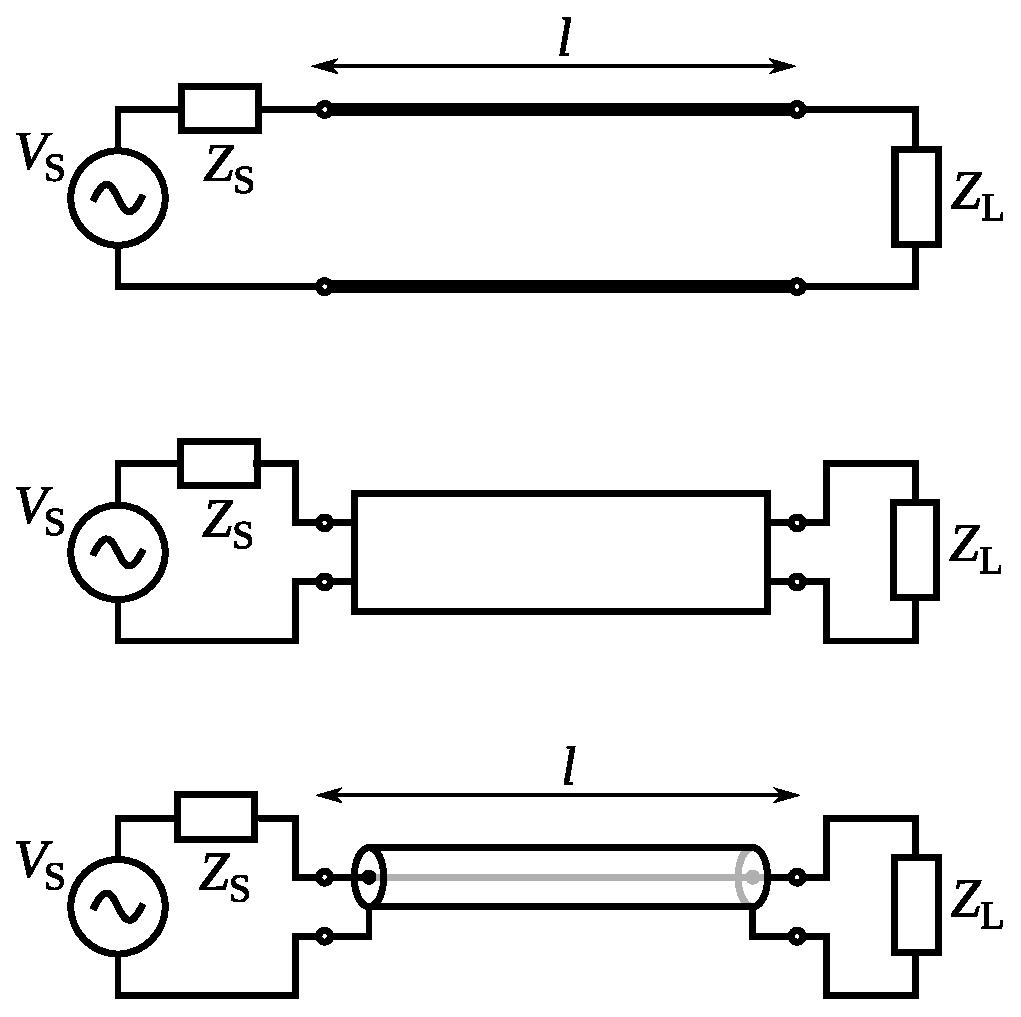
\includegraphics[width=\columnwidth]{modules/m0077_Transmission_line_symbols_se170804.eps}
% https://commons.wikimedia.org/wiki/File:Transmission_line_symbols.svg
}}{Three circuit diagrams depicting a generic two-conductor direct connection (top), a generic two port "black box" (middle), and a coaxial cable (bottom). The top diagram consists of a rectangular series circuit with a circle with a curved line in it representing the voltage source (V sub s) on the left. A source impedance (Z sub s) is represented by a small rectangle to the right of source. A load impedance (Z sub L) is represented by a small rectangle on the right side of the circuit. V sub s, Z sub s, and Z sub L are identically placed in the other two diagrams. On the top and bottom of the rectangle, a thicker line labeled "l" represents the length of the transmission line.  The middle diagram shows another rectangle laid over the middle of the circuit representing a two-port "black box." The bottom diagram depicts a cylinder laid over the middle of the circuit, with the circuit going through it, to represent a coaxial cable.}
\end{center} 
\centerline{\scriptsize 
\copyright~\hyperref[m0077_fTransmission_line_symbols_Credit]{Omegatron}
\href{https://creativecommons.org/licenses/by-sa/3.0/deed.en}{CC BY~SA 3.0 Unported} (modified) 
} 
\caption{
\label{m0077_fTransmission_line_symbols}
Symbols representing transmission lines: 
\emph{Top}: As a generic two-conductor direct connection.
\emph{Middle}: As a generic two-port ``black box.''
\emph{Bottom}: As a coaxial cable. 
}
\end{figure}

The two-port representation
\index{two-port}
of a transmission line is completely described by its length $l$ along with some combination of the following parameters: 
%
\begin{itemize}
\item Phase propagation constant $\beta$, 
\index{propagation constant!phase}
having units of rad/m.  This parameter also represents the wavelength in the line through the relationship $\lambda=2\pi/\beta$.
(See Sections~\ref{m0074_Fundamentals_of_Waves} and \ref{m0080_Wave_Propagation_on_a_Transmission_Line} for details.)
\item Attenuation constant $\alpha$, 
\index{propagation constant!attenuation}
having units of 1/m. This parameter quantifies the effect of loss in the line.
(See Section~\ref{m0080_Wave_Propagation_on_a_Transmission_Line} for details.)
\item Characteristic impedance $Z_0$, 
\index{characteristic impedance}
\index{impedance!characteristic|see{characteristic impedance}}
having units of $\Omega$.  This is the ratio of potential (``voltage'') to current when the line is perfectly impedance-matched at both ends.
(See Section~\ref{m0052_Characteristic_Impedance} for details.)  
\end{itemize}
These parameters depend on the materials and geometry of the line.

Note that a transmission line is typically not transparent to the source and load.
In particular, the load impedance may be $Z_L$, but the impedance presented to the source may or may not be equal to $Z_L$.
(See Section~\ref{m0087_Input_Impedance_of_a_Terminated_Lossless_Transmission_Line} for more on this concept.)
Similarly, the source impedance may be $Z_S$, but the impedance presented to the load may or may not be equal to $Z_S$.
The effect of the transmission line on the source and load impedances will depend on the parameters identified above.

%%%%%%%%%%%%%%%%%%%%%%%%%%%%%%%%

{\bf Additional Reading:}
\begin{itemize}
\item ``\href{https://en.wikipedia.org/wiki/Thevenin's_theorem}{Th\'{e}venin's theorem}'' on Wikipedia.
\end{itemize}

\index{transmission line!two-port representation|)}

